\section{问题三的模型建立与求解}
\subsection{聚类分析确定打包方案}
问题三考虑到将位置较为集中的任务联合打包发布,从而提高了任务完成的
效率。因此,我们首先需要根据任务的位置信息判断哪些任务的位置分布较为集
中,从而确定打包方案。附件一给出的任务位置信息即为经纬度数据,首先,将
经纬度的数据作为地理位置的定量分析数据,利用聚类分析的方法,从位置分布
上对任务进行准确、细致的分类。此时,位置分布比较集中的任务会被自动归为
一类。我们将分析聚类结果的合理性,对于合理的分类,直接将此类中的任务联
合打包。对于不合理的分类,我们将对分类结果进一步调整后再打包。

Step 1:第一层聚类分析

首先,我们对聚类分析的分类数进行大致估算,由于任务总数为845 个,将
任务按照位置信息分为150 类时,平均每一类大约有5—6 个任务,这个数值比
较合理。因此,初次聚类时,将任务的位置分布分为150 类,利用Matlab 的
K-Means 命令得到的聚类分析图:

\begin{figure}[H]
    \centering
    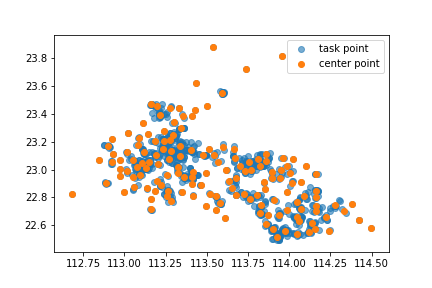
\includegraphics[width=1\textwidth]{150.png}
    \caption{K-Means聚类分析图}
    \label{}
\end{figure}

任务打包方案应当考虑两方面的问题:一是联合打包的任务应该在位置分布
上较为集中;二是一个任务包内的任务数量应当合理。我们假设一个任务包内的
任务数量取值范围为[2,15]。该聚类结果保证了一类中的任务在位置分布上较为
集中,下面来分析每个任务包中的任务数量是否符合假设。

我们依据任务的位置信息将任务按照分布的集中度分成150 类,最多的类别
中有18 个任务。最少的类别中只有1 个任务。对于一类中只有1 个的任务,由
于其位置分布偏散,我们不对其做打包处理。但对于任务个数大于15 个的类别,
我们将这些任务位置信息提取出来,进行二次聚类分析。

Step 2:第二层聚类分析

我们假设当一类中任务数量不超过15 个时,这个打包方案才是合理的,在
上述聚类分析中,有九个类别中的任务数量超过了15 个.

对于这九个不合理的分类,我们在第一次分类结果的基础上,进行嵌套的聚
类分析,将它们分成两类。将这九个分类中的任务位置信息提取出来,再一次根
据其经纬度数据,利用Matlab 的K-Means 命令进行第二层聚类分析。
分别得到如下的分类图:

\begin{figure}
    \centering
    \begin{minipage}[c]{0.3\textwidth}
        \centering
        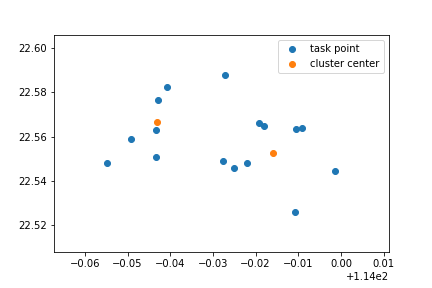
\includegraphics[width=0.95\textwidth]{24.png}
        \subcaption{第24类二次聚类图}
        \label{fig:sample-figure-a}
    \end{minipage}
    \begin{minipage}[c]{0.3\textwidth}
        \centering
        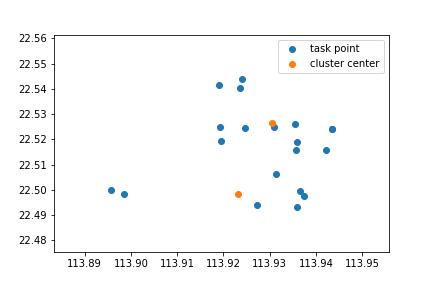
\includegraphics[width=0.95\textwidth]{25.png}
        \subcaption{第25类二次聚类图}
        \label{fig:sample-figure-b}
    \end{minipage}
    \begin{minipage}[c]{0.3\textwidth}
        \centering
        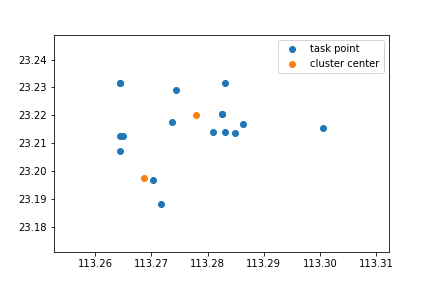
\includegraphics[width=0.95\textwidth]{83.png}
        \subcaption{第83类二次聚类图}
        \label{fig:sample-figure-c}
    \end{minipage}\\
    \begin{minipage}[c]{0.3\textwidth}
        \centering
        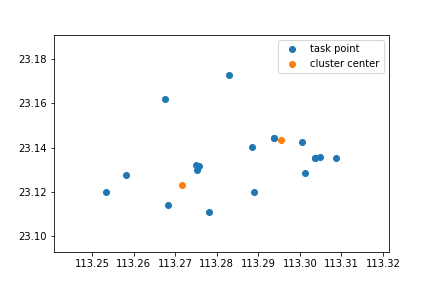
\includegraphics[width=0.95\textwidth]{96.png}
        \subcaption{第96类二次聚类图}
        \label{fig:sample-figure-a}
    \end{minipage}
    \begin{minipage}[c]{0.3\textwidth}
        \centering
        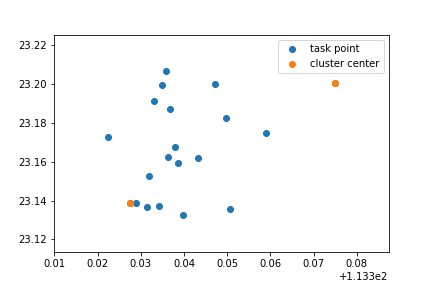
\includegraphics[width=0.95\textwidth]{113.png}
        \subcaption{第113类二次聚类图}
        \label{fig:sample-figure-b}
    \end{minipage}
    \begin{minipage}[c]{0.3\textwidth}
        \centering
        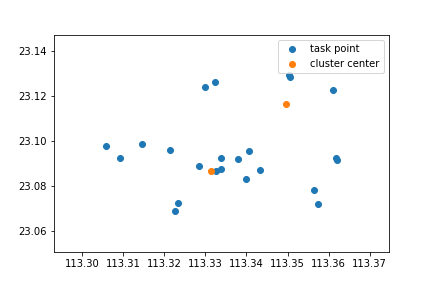
\includegraphics[width=0.95\textwidth]{120.png}
        \subcaption{第120类二次聚类图}
        \label{fig:sample-figure-c}
    \end{minipage}\\    \begin{minipage}[c]{0.3\textwidth}
        \centering
        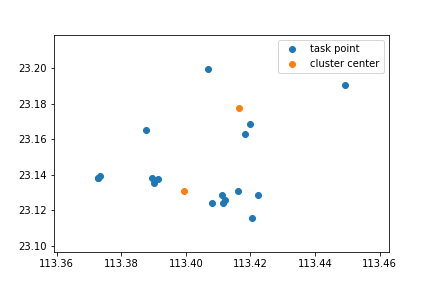
\includegraphics[width=0.95\textwidth]{128.png}
        \subcaption{第128类二次聚类图}
        \label{fig:sample-figure-a}
    \end{minipage}
    \begin{minipage}[c]{0.3\textwidth}
        \centering
        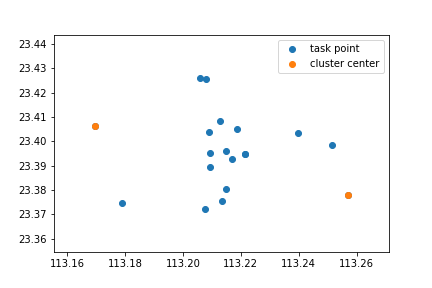
\includegraphics[width=0.95\textwidth]{140.png}
        \subcaption{第140类二次聚类图}
        \label{fig:sample-figure-b}
    \end{minipage}
    \begin{minipage}[c]{0.3\textwidth}
        \centering
        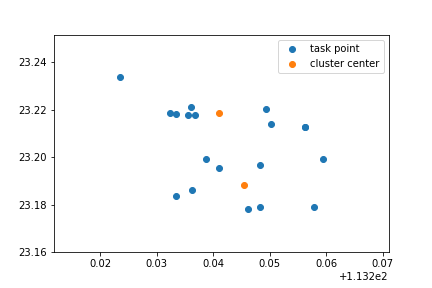
\includegraphics[width=0.95\textwidth]{141.png}
        \subcaption{第141类二次聚类图}
        \label{fig:sample-figure-c}
    \end{minipage}\\
    \caption{二重嵌套聚类分析图}
    \label{fig:sample-figure}
\end{figure}

对这九个类别进行嵌套聚类分析后,每一类别都由两个小类组成,每一小类
包含的任务数量由下面的统计表格给出:
% Please add the following required packages to your document preamble:
% \usepackage{multirow}
% \usepackage{longtable}
% Note: It may be necessary to compile the document several times to get a multi-page table to line up properly
\begin{longtable}[c]{ccc}
    \caption{嵌套聚类后任务数量}
    \label{tab:my-table}\\
    \hline
    类号                   & 新类别 & 再计数 \\ \hline
    \endfirsthead
    %
    \endhead
    %
    \multirow{2}{*}{24}  & 1   & 9   \\
                         & 2   & 7   \\ \hline
    \multirow{2}{*}{25}  & 1   & 7   \\
                         & 2   & 13  \\ \hline
    \multirow{2}{*}{83}  & 1   & 3   \\
                         & 2   & 14  \\ \hline
    \multirow{2}{*}{96}  & 1   & 8   \\
                         & 2   & 11  \\ \hline
    \multirow{2}{*}{113} & 1   & 12  \\
                         & 2   & 8   \\ \hline
    \multirow{2}{*}{120} & 1   & 7   \\
                         & 2   & 15  \\ \hline
    \multirow{2}{*}{128} & 1   & 5   \\
                         & 2   & 13  \\ \hline
    \multirow{2}{*}{140} & 1   & 12  \\
                         & 2   & 7   \\ \hline
    \multirow{2}{*}{141} & 1   & 10  \\
                         & 2   & 9   \\ \hline
    \end{longtable}
嵌套聚类分析后,每一类别的任务数量符合要求,此时得到的分类方案合理。


Step 3:确定任务打包方案

根据上述两次基于任务位置分布的聚类分析结果,我们将位置分布较为集中
的任务联合打包,同时保证每一个任务包内的任务数量不多于15 个,得到了一
个合理、准确的任务打包方案。

将一个任务包里的多个任务看做一个整体,与其它未被打包的任务同为一个
任务,经过联合打包处理过后的任务数量由835 个变为154 个。
